\documentclass[10pt]{beamer}

\usetheme[progressbar=frametitle]{metropolis}

\usepackage{booktabs}
\usepackage[scale=2]{ccicons}


\usepackage{amsmath}
\usepackage{pgfplots}
\usepgfplotslibrary{dateplot}

\usepackage{xspace}
\newcommand{\themename}{\textbf{\textsc{metropolis}}\xspace}

%\usepackage{placeins} %%%
\usepackage{subfig}
\usepackage{physics}
\usepackage{amssymb}


\usepackage{tikz}
\usepackage{circuitikz}
\usepackage{siunitx}


\usepackage{latexsym}
\usepackage{mathtools}
\usepackage{slashed} % for the Feynman slash notation

\usepackage{listings}

\usepackage{balance}


% edited by Mauro 28-12-16
%
%% <local definitions>
\newcommand{\R}{\mathbb{R}}	
\newcommand{\C}{\mathbb{C}}
\newcommand{\HQ}{\mathbb{H}}
\newcommand{\N}{\mathbb{N}}
\newcommand{\be}{\begin{equation}}
\newcommand{\ee}{\end{equation}}	
\newcommand{\bea}{\begin{eqnarray}}
\newcommand{\eea}{\end{eqnarray}}	
\newcommand{\Pin}{\mathrm{Pin}}	
\newcommand{\Spin}{\mathrm{Spin}}
\renewcommand{\O}{\mathrm{O}}
\newcommand{\SO}{\mathrm{SO}}
\renewcommand{\eqref}[1]{(\ref{#1})}
\newcommand{\cl}[1]{\ensuremath{Cl(#1)}} % #1 stands for the values p,q. $\cl{p,q}$ produces 'Cl(p,q)'.
\newcommand{\gvec}[1]{\ensuremath{\mbox{\textbf{\textit{#1}}}}}
\newcommand{\vect}[1]{\ensuremath{\mbox{\textbf{\textit{#1}}}}}
%% </local definitions>

\newcommand{\Ba}[0]{\mathbf{a}}
\newcommand{\Bb}[0]{\mathbf{b}}
\newcommand{\Bc}[0]{\mathbf{c}}
\newcommand{\Bd}[0]{\mathbf{d}}
\newcommand{\Be}[0]{\mathbf{e}}
\newcommand{\Bf}[0]{\mathbf{f}}
\newcommand{\Bg}[0]{\mathbf{g}}
\newcommand{\Bh}[0]{\mathbf{h}}
\newcommand{\Bi}[0]{\mathbf{i}}
\newcommand{\Bj}[0]{\mathbf{j}}
\newcommand{\Bk}[0]{\mathbf{k}}
\newcommand{\Bl}[0]{\mathbf{l}}
\newcommand{\Bm}[0]{\mathbf{m}}
\newcommand{\Bn}[0]{\mathbf{n}}
\newcommand{\Bo}[0]{\mathbf{o}}
\newcommand{\Bp}[0]{\mathbf{p}}
\newcommand{\Bq}[0]{\mathbf{q}}
\newcommand{\Br}[0]{\mathbf{r}}
\newcommand{\Bs}[0]{\mathbf{s}}
\newcommand{\Bt}[0]{\mathbf{t}}
\newcommand{\Bu}[0]{\mathbf{u}}
\newcommand{\Bv}[0]{\mathbf{v}}
\newcommand{\Bw}[0]{\mathbf{w}}
\newcommand{\Bx}[0]{\mathbf{x}}
\newcommand{\By}[0]{\mathbf{y}}
\newcommand{\Bz}[0]{\mathbf{z}}
\newcommand{\BA}[0]{\mathbf{A}}
\newcommand{\BB}[0]{\mathbf{B}}
\newcommand{\BC}[0]{\mathbf{C}}
\newcommand{\BD}[0]{\mathbf{D}}
\newcommand{\BE}[0]{\mathbf{E}}
\newcommand{\BF}[0]{\mathbf{F}}
\newcommand{\BG}[0]{\mathbf{G}}
\newcommand{\BH}[0]{\mathbf{H}}
\newcommand{\BI}[0]{\mathbf{I}}
\newcommand{\BJ}[0]{\mathbf{J}}
\newcommand{\BK}[0]{\mathbf{K}}
\newcommand{\BL}[0]{\mathbf{L}}
\newcommand{\BM}[0]{\mathbf{M}}
\newcommand{\BN}[0]{\mathbf{N}}
\newcommand{\BO}[0]{\mathbf{O}}
\newcommand{\BP}[0]{\mathbf{P}}
\newcommand{\BQ}[0]{\mathbf{Q}}
\newcommand{\BR}[0]{\mathbf{R}}
\newcommand{\BS}[0]{\mathbf{S}}
\newcommand{\BT}[0]{\mathbf{T}}
\newcommand{\BU}[0]{\mathbf{U}}
\newcommand{\BV}[0]{\mathbf{V}}
\newcommand{\BW}[0]{\mathbf{W}}
\newcommand{\BX}[0]{\mathbf{X}}
\newcommand{\BY}[0]{\mathbf{Y}}
\newcommand{\BZ}[0]{\mathbf{Z}}

\newcommand{\ta}[0]{\tilde{a}}
\newcommand{\tb}[0]{\tilde{b}}
\newcommand{\tc}[0]{\tilde{c}}
\newcommand{\td}[0]{\tilde{d}}

\newcommand{\hA}[0]{\hat{A}}
\newcommand{\hB}[0]{\hat{B}}
\newcommand{\hH}[0]{\hat{H}}

\newcommand{\tA}[0]{\tilde{A}}
\newcommand{\tB}[0]{\tilde{B}}
\newcommand{\tF}[0]{\tilde{F}}
\newcommand{\tE}[0]{\tilde{E}}
\newcommand{\tH}[0]{\tilde{H}}

% spinors definition
\newcommand{\barJ}[0]{\bar{J}}
\newcommand{\barF}[0]{\bar{F}}
\newcommand{\barP}[0]{\bar{P}}
\newcommand{\barW}[0]{\bar{W}}



\newcommand{\tnabla}[0]{\tilde{\nabla}}
\newcommand{\tphi}[0]{\tilde{\phi}}
\newcommand{\tpsi}[0]{\tilde{\psi}}

%
\newcommand{\wavep}[0]{\partial^+}
\newcommand{\wavem}[0]{\partial^-}

\newcommand{\wavepp}[0]{\tilde{\partial}^+}
\newcommand{\wavemp}[0]{\tilde{\partial}^-}

\newcommand{\wavepd}[0]{\bar{\partial}^+}
\newcommand{\wavemd}[0]{\bar{\partial}^-}

\newcommand{\pbd}[0]{\bar{\partial}_d}

% frequency

\newcommand{\helmp}[0]{{\underline{\partial}}^+}
\newcommand{\helmm}[0]{{\underline{\partial}}^-}

\newcommand{\helmpp}[0]{{\underline{\tilde{\partial}}}^+}
\newcommand{\helmmp}[0]{{\underline{\tilde{\partial}}}^-}

\newcommand{\helmpd}[0]{{\underline{\bar{\partial}}}^+}
\newcommand{\helmmd}[0]{{\underline{\bar{\partial}}}^-}

\newcommand{\pbfd}[0]{{\underline{\bar{\partial}}}_d}




\def \figname {Figure}
\def \emode {E }
\def \hmode {H }
\def \temode {TE }
\def \tmmode {TM }
\def \temoden {TE${}_n$ }
\def \tmmoden {TM${}_n$ }
\def \temodemn {TE${}_{mn}$ }
\def \tmmodemn {TM${}_{mn}$ }



\newcommand{\iGA}{{i}}
\newcommand{\conjg}[1] {\ensuremath{#1}^*}

\setbeamertemplate{bibliography item}{[\theenumiv]}


\title{Frequency Spectrum}

\date{}

%\subtitle{Maximizing efficiency and power at a fixed frequency}
%\date{\today}
%\author{Alessandra Costanzo, Franco Mastri, Mauro Mongiardo*, Giuseppina Monti}
%\institute{*Department of Engineering,
%University of Perugia, Italy}

\author{ Mauro Mongiardo$^1$}

\institute{ $^1$ Department of Engineering, University of Perugia, Perugia, Italy.
}

%
\titlegraphic{\hfill\includegraphics[height=1.5cm]{logo}}


\begin{document}

\maketitle

\begin{frame}{Table of contents}
  \setbeamertemplate{section in toc}[sections numbered]
  \tableofcontents[hideallsubsections]
\end{frame}


\def\EMspectrum{\centering
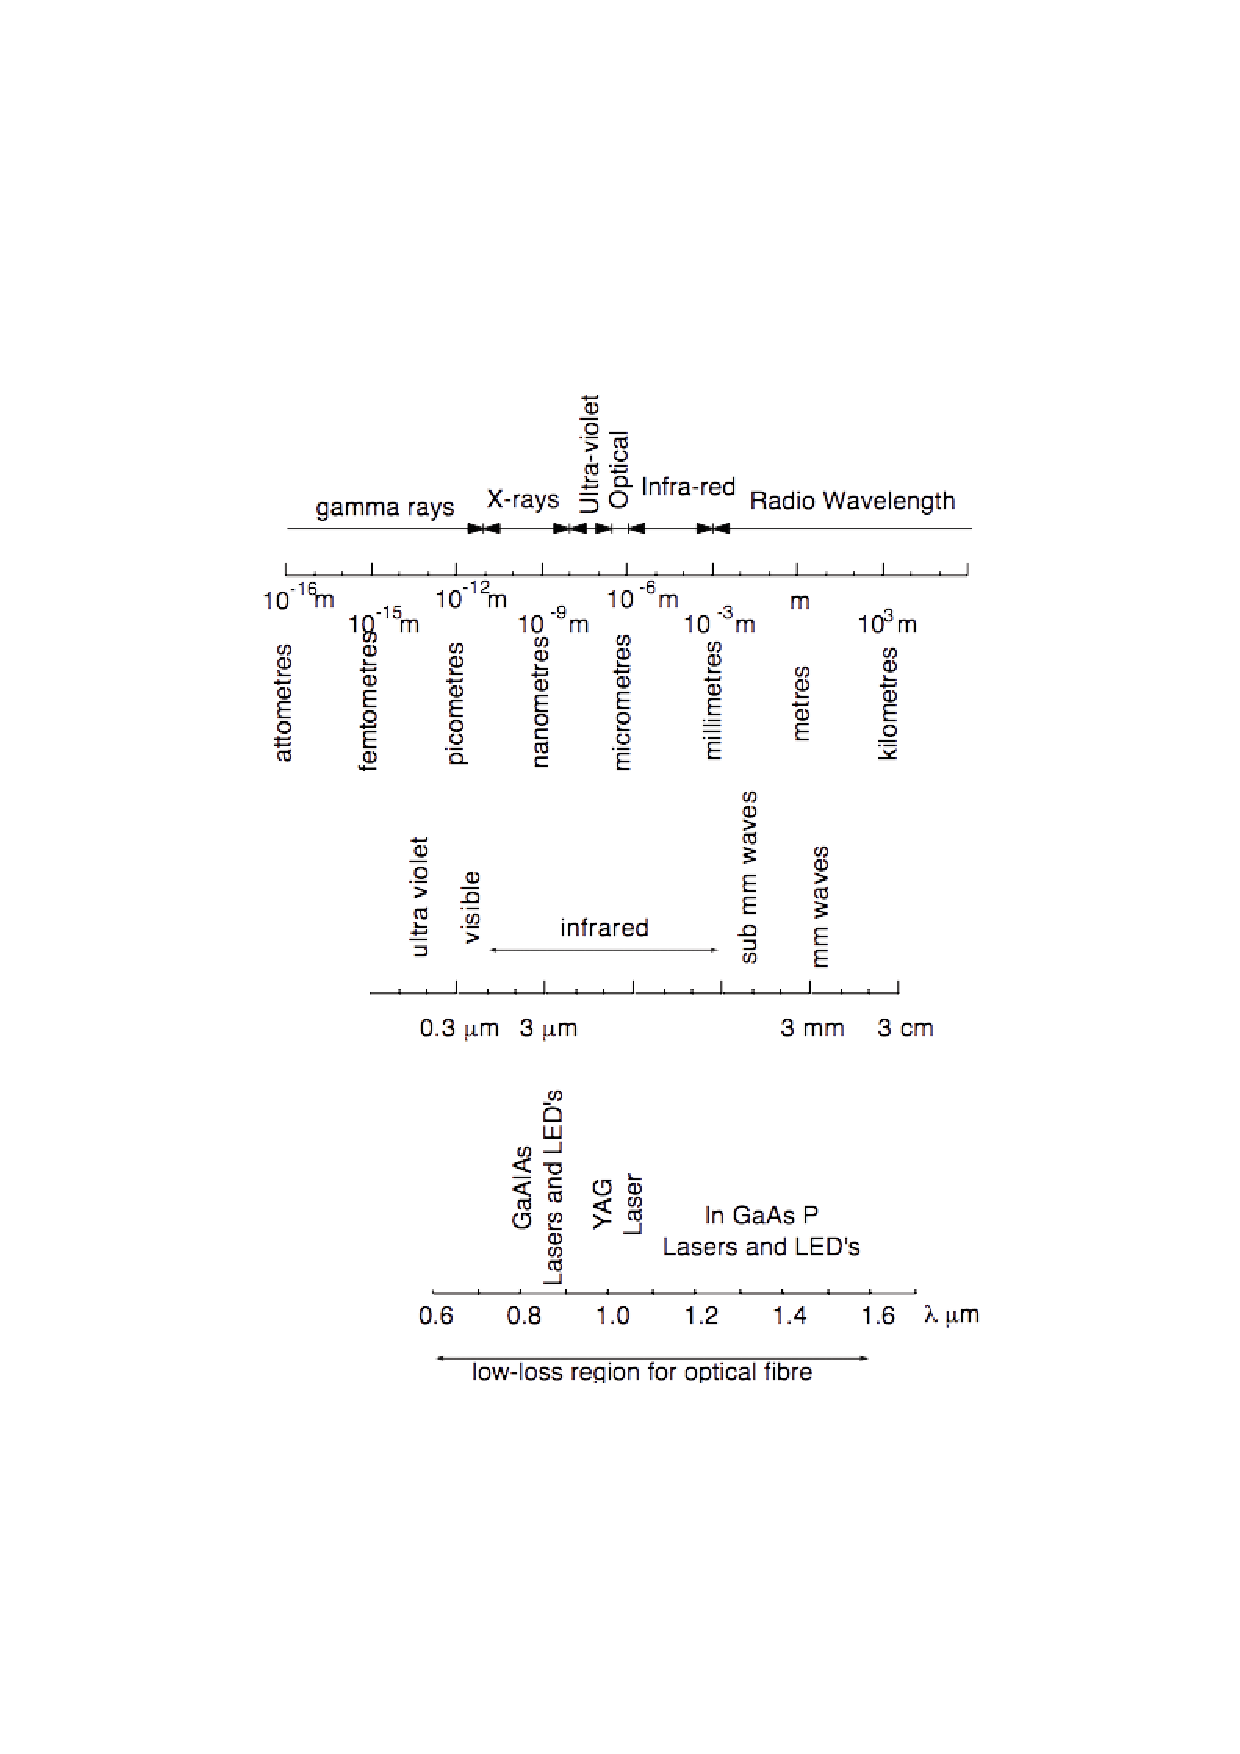
\includegraphics[width=0.75\textwidth]{EMspectrum}}

\def\atmatt{\centering
\includegraphics[width=0.75\textwidth]{atmatt3.eps}}


%



%=========================================================================
\section{The frequency spectrum}
%=========================================================================


%=========================================================================
\begin{frame}[fragile]{}
%
The \href{https://en.wikipedia.org/wiki/Electromagnetic_spectrum}{\textcolor{blue}{Electromagnetic frequency  spectrum}}
  %electromagnetic frequency  spectrum 
  is  represented in
Figure \ref{EMspectrum} in terms of the wavelength. 

In this
Figure is also shown the portion of spectrum where the
transmission characteristics of optical fibers are best
utilized.  

Waveguides used in optical communication
systems and in integrated optics are generally operated in this
frequency range. 

Another part of the spectrum intensively used is
that corresponding to radio wavelengths, as detailed in
Table~\ref{band} 
%\cite{Collin:ant}

\end{frame}
%=========================================================================
\begin{frame}[shrink=10]{Electromagnetic wave spectrum}
\begin{figure}[tb]
\EMspectrum
\caption{Electromagnetic wave spectrum.}
\label{EMspectrum} 
\end{figure}
%\vfill
%\index{electromagnetic spectrum}   

\end{frame}

%%=========================================================================
\begin{frame}[shrink=60]{}
%

\begin{table}
%
\caption{Radio frequency band designations and use.}
\vspace{0.1in}
\center
%
\begin{tabular}{|c | c | p{0.75in} | p{1.4in}|}  \hline 
{\em Frequency} & {\em Wavelength} & \centering{\em {Band designation}} & {\em Typical
service }\\
\hline \hline
 30-300  Hz &  10-1 Mm    &  \centering{ELF} & \\ 
300-3000 Hz & 1000-100 km &  \centering{extremely low frequency} & \\ \hline

3-30 kHz    & 100-10  km  &    \centering {VLF \\ very low frequency} 
&  \parbox[t]{1.4in} {\small Navigation, sonar}  \\ \hline
                   
30-300  kHz &  10-1 km    & \centering{ LF \\ low frequency} &
  \parbox[t]{1.4in}{\small Radio beacons, \hfill navigational aids}    \\ \hline

300-3000  kHz &1 km-100 m   &   \centering{MF \\ medium frequency} 
&  \parbox[t]{1.4in}{\small AM broad\-cas\-ting, maritime radio, Coast Guard communication,
\hfill direction finding} \\ \hline

3-30 MHz	&100-10 m &	\centering{HF \\ high frequency}
 &  \parbox[t]{1.4in}{\small Telephone, \hfill telegraph, facsimile; shortwave international
broadcasting; amateur radio; citizen's band; ship to coast and ship to aircraft
communication}   \\
\hline

30-300 MHz	& 10-1 m &	\centering{VHF \\ very high frequency}
 & \parbox[t]{1.4in} {\small Television, \hfill FM broadcast, air traffic control, police,
taxicab mobile radio,  navigational aids}  \\ \hline

300-3000 MHz	& 1 m-10 cm &	\centering{UHF \\ ultra high frequency} 
&  \parbox[t]{1.4in}{\small Television, \hfill radioprobes,
satellite communication, surveillance radar,
 navigational aids} \\ \hline

3-30 GHz &	10-1 cm &	\centering{SHF \\ super high frequency} 
&  \parbox[t]{1.4in} {\small Airborne radar, satellite communication, common carrier land
mobile communication, \hfill
 micro\-wave links} \\ \hline

30-300 GHz &	1 cm- 1 mm &	\centering{EHF \\ extremely high frequency}
 &  \parbox[t]{1.4in}{\small Experimental, \hfill Radar,
\hfill vehicular \hfill anti-collision radar }
\\
\hline
% 300-3000 GHz &	1 mm-100 mm &	 &  \\ \hline
%\hline \hline
\end{tabular}
\normalsize
%\caption{Radio frequency band designations and use.}
\label{band}
\end{table}

\end{frame}
%%=========================================================================
\begin{frame}[fragile]{}
%
\alert{Electromagnetic communications can take place in free--space or with guided waves}.

Waveguides
operating at microwave and millimeter waves  are of
particular interest for their wide range of applications.

The frequency band designations employed in the microwave
range are reported in Table~\ref{IEEEband}.

\end{frame}
%%=========================================================================
\begin{frame}[fragile]{}
%

\begin{table}[bt]
\caption{Microwave frequency band designations.}
\vspace{0.1in}
\center
\small
%
\begin{tabular}{ c c c c } \hline \hline
\multicolumn{1}{c}{Frequency} &	\multicolumn{1}{c}{Wavelength} &	
\multicolumn{2}{c}{IEEE radar band designation} \\ \cline{3-4} 
              &                & old & new \\ \hline
1-2 GHz      	& 30-15 cm        &	L  & D    \\
2-3  GHz	     & 15-10 cm        &	S  & E   \\
3-4  GHz	     & 10-7.5 cm       &	S  & F   \\
4-6 GHz      	&  7.5-5 cm       &	C  & G   \\
6-8 GHz      	&  5-3.75 cm      &	C  & H   \\
8-10 GHz	     &  3.75-3 cm      &	X  & I   \\
10-12.4 GHz	  &  3-2.42 cm      &	X  & J   \\
12.4-18 GHz  	&  2.42-1.67 cm   &	Ku & J   \\
18-20 GHz    	&  1.67-1.5 cm    &	K  & J    \\
20-26.5 GHz  	&  1.5-1.13 cm    &	K  & K  \\
26.5-40 GHz  	&  1.13 cm-7.5 mm &	Ka & K  \\
40-300 GHz   	&  7.5-1.0 mm     &	mm &    \\
\hline \hline
\end{tabular}
\normalsize
%\caption{Microwave frequency band designations.}
\label{IEEEband}
\end{table}
%\vfill

\end{frame}
%%=========================================================================
\begin{frame}[fragile]{wavenumber concept}
%
The \alert{wavenumber} concept  is 
perhaps more   fundamental  in  electromagnetic  wave
theory   than  either  of  the  more  popular
concepts  of  \alert{wavelength and  frequency}.  

The
corresponding   values   of   wavenumber $k$ and
frequency $f$  are obtained from the wavelength $\lambda$ by
the following relationships
%
\begin{eqnarray}
f = {c \over \lambda} & & \lambda={2 \pi \over k}
\end{eqnarray}
%
where $c$ is the free--space velocity of light, \index{light
velocity}
%

%
\begin{eqnarray}
c = {1 \over 
 \sqrt{ \mu_{0} \varepsilon_{0} } } = 2.997925 \times 10^{8} 
 \mbox{m/s}
 \approx 3 \times 10^{8} \mbox{m/s}  & & \nonumber \\
%
\end{eqnarray}
and
 
%
\end{frame}
%%=========================================================================
\begin{frame}[fragile]{}
%
\begin{eqnarray}
{\mu}_{0} = 4 \pi \times 10^{-7} henry/metre & 
 & \left( {V \cdot s \over A \cdot m} \right) \nonumber \\
%
 \varepsilon_{0} = {1 \over 36 \pi} \times 10^{-9} farad/metre
& & \left( {A \cdot s \over V \cdot m} \right) 
\label{permittivity}
\end{eqnarray}

%
%
where  

$\mu_{0}$ is the magnetic permeability 

$\varepsilon_{0}$ the  dielectric permittivity of 
free--space. 
%\index{magnetic permeability} \index{dielectric permittivity}
\end{frame}
%%=========================================================================
\begin{frame}[fragile]{Guided waves}
%
Waveguides may operate up to optical
frequencies. 

For communication  purposes, since
it   is   generally desirable to employ  as \alert{large a
bandwidth}  as possible, it is
advantageous  to use  the higher frequencies
now available. 

Up to the millimetric range this is an added 
bonus, as \alert{circuit  dimensions   become   smaller   as frequency
increases}, thus allowing  a  saving of  space
and sometimes a reduction of  costs when higher
frequencies are used.

\end{frame}

\section{Atmospheric attenuation}
%%=========================================================================
\begin{frame}[fragile]{Atmospheric attenuation}
%
\alert{As frequency increases so
does the average atmospheric attenuation},  as
shown in Figure \ref{EMattenuation} 
 
This fact,  together  with   problems
related   to   electromagnetic  interference,
 \alert{prevents   the use of 
free--space   as   a transmitting  media for very large  amounts 
of data}.   

\alert{Atmospheric   attenuation   is   also
important for many applications}; for example,
by   choosing  frequencies  for   which   the
atmosphere is opaque, one prevents  detection
of  satellite--to--satellite communications  by
ground--based      receivers.       

Similarly,
terrestrial  systems  desiring   to   prevent
signal  overshoot in range may operate  at  a
frequency   of  high  atmospheric  absorption
%\cite{Wiltse}

\end{frame}
%=========================================================================
\begin{frame}[fragile]{Attenuation by oxygen  and water vapour}
%
\begin{figure}[tb]
\atmatt
\caption{Attenuation by oxygen (dotted line) and water vapour
         (continuous line) at sea
         level. The water content is 7.5 $g/m^{3}$ and the
         temperature is T = 20$^{\circ}$C.}
\label{EMattenuation} 
\end{figure}
\end{frame}

%=========================================================================
\section{Computation example}
%=========================================================================
\begin{frame}[fragile]{Speed of light frequency and wavelength}
The frequency $f$, the wavelength $\lambda$ and the speed of light $c$ are also related by the \alert{important relation
\be
c = f \lambda
\ee
}
As an example compute the wavelength of a gps receiver with $f=$ \SI{ 1575.42} {\mega \hertz} 

\end{frame}

%%=========================================================================
\begin{frame}[shrink=40]{}

The  code clf.wxm computes wavelength from frequency.
% The file 
%\small
%\begin{verbatim}
%clf.wxm
%\end{verbatim}
%\normalsize
%
%is listed in the following.

\small
\lstinputlisting{clf.wxm}
\normalsize


\end{frame}



%%=========================================================================
%\begin{frame}[fragile]{}
%
%\end{frame}
%%=========================================================================
%\begin{frame}[fragile]{}
%
%\end{frame}
%%=========================================================================
%\begin{frame}[fragile]{}
%
%\end{frame}
%%=========================================================================
%\begin{frame}[fragile]{}
%
%\end{frame}
%%=========================================================================
%\begin{frame}[fragile]{}
%
%\end{frame}
%%=========================================================================
%\begin{frame}[fragile]{}
%
%\end{frame}
%




\end{document}
